\begin{figure}[htbp]
\centering
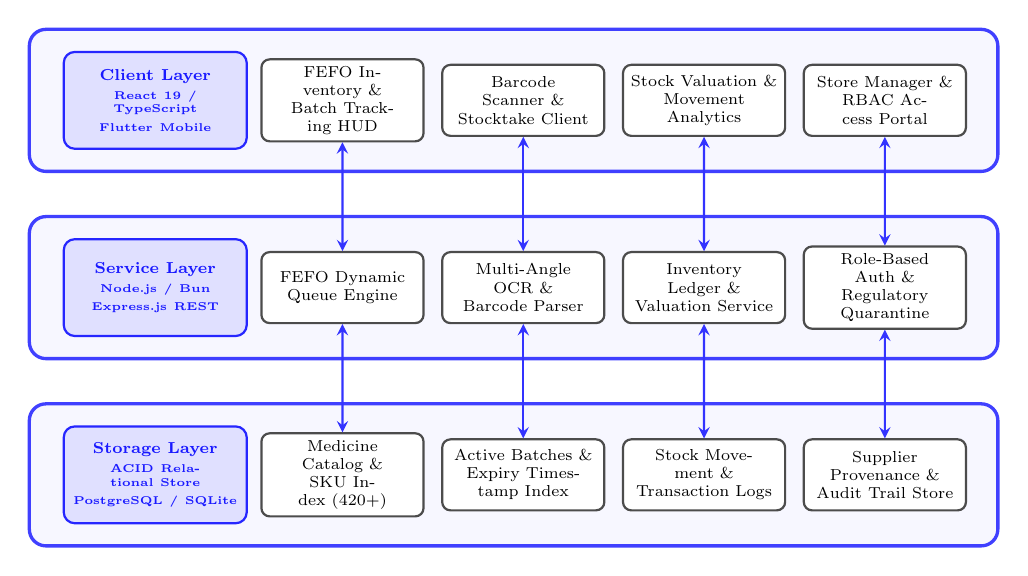
\begin{tikzpicture}[
    scale=0.82, every node/.style={transform shape},
    layer/.style={rectangle, draw=blue!75, fill=blue!3, very thick, rounded corners=6pt, minimum width=15.0cm, minimum height=2.2cm},
    tierbadge/.style={rectangle, draw=blue!85, fill=blue!12, thick, rounded corners=4pt, minimum width=2.8cm, text width=2.6cm, minimum height=1.5cm, font=\bfseries\scriptsize, align=center, text=blue!90},
    submodule/.style={rectangle, draw=black!70, fill=white, thick, rounded corners=3pt, minimum width=2.4cm, text width=2.3cm, minimum height=1.1cm, font=\scriptsize, align=center, inner sep=3pt}
]

% ==================== CLIENT PRESENTATION LAYER ====================
\node[layer] (clientlayer) at (-0.45, 4.4) {};
\node[tierbadge] (tb_c) at (-6.0, 4.4) {Client Layer\\[0.08cm]\tiny React 19 / TypeScript\\Flutter Mobile};
\node[submodule] (sub_c1) at (-3.1, 4.4) {FEFO Inventory \&\\Batch Tracking HUD};
\node[submodule] (sub_c2) at (-0.3, 4.4) {Barcode Scanner \&\\Stocktake Client};
\node[submodule] (sub_c3) at (2.5, 4.4) {Stock Valuation \&\\Movement Analytics};
\node[submodule] (sub_c4) at (5.3, 4.4) {Store Manager \&\\RBAC Access Portal};

% ==================== APPLICATION & SERVICE LAYER ====================
\node[layer] (servicelayer) at (-0.45, 1.5) {};
\node[tierbadge] (tb_s) at (-6.0, 1.5) {Service Layer\\[0.08cm]\tiny Node.js / Bun\\Express.js REST};
\node[submodule] (sub_s1) at (-3.1, 1.5) {FEFO Dynamic\\Queue Engine};
\node[submodule] (sub_s2) at (-0.3, 1.5) {Multi-Angle OCR \&\\Barcode Parser};
\node[submodule] (sub_s3) at (2.5, 1.5) {Inventory Ledger \&\\Valuation Service};
\node[submodule] (sub_s4) at (5.3, 1.5) {Role-Based Auth \&\\Regulatory Quarantine};

% ==================== PERSISTENCE & STORAGE LAYER ====================
\node[layer] (datalayer) at (-0.45, -1.4) {};
\node[tierbadge] (tb_d) at (-6.0, -1.4) {Storage Layer\\[0.08cm]\tiny ACID Relational Store\\PostgreSQL / SQLite};
\node[submodule] (sub_d1) at (-3.1, -1.4) {Medicine Catalog \&\\SKU Index (420+)};
\node[submodule] (sub_d2) at (-0.3, -1.4) {Active Batches \&\\Expiry Timestamp Index};
\node[submodule] (sub_d3) at (2.5, -1.4) {Stock Movement \&\\Transaction Logs};
\node[submodule] (sub_d4) at (5.3, -1.4) {Supplier Provenance \&\\Audit Trail Store};

% ==================== VERTICAL COMMUNICATION PIPELINES ====================
% Layer 1 <-> Layer 2
\draw[thick, <->, >=stealth, blue!80] (sub_c1) -- (sub_s1);
\draw[thick, <->, >=stealth, blue!80] (sub_c2) -- (sub_s2);
\draw[thick, <->, >=stealth, blue!80] (sub_c3) -- (sub_s3);
\draw[thick, <->, >=stealth, blue!80] (sub_c4) -- (sub_s4);

% Layer 2 <-> Layer 3
\draw[thick, <->, >=stealth, blue!80] (sub_s1) -- (sub_d1);
\draw[thick, <->, >=stealth, blue!80] (sub_s2) -- (sub_d2);
\draw[thick, <->, >=stealth, blue!80] (sub_s3) -- (sub_d3);
\draw[thick, <->, >=stealth, blue!80] (sub_s4) -- (sub_d4);

\end{tikzpicture}
\caption{Three-Tier Architectural Decomposition of the Kaziniya PIMS Platform.}
\label{fig:sys_arch}
\end{figure}
